
\section{Heap}

To model the memory used by the program we want to verify, we use a graph with nodes and labeled edges.
Each node represents a memory cell whereas each edge represents a pointer to the next part of the Data-Structure.
The edges are labeled with a color to distinguish between these selectors. For simplicity only structures with
two pointers will be considered. The selectors will be labeled 1 and 2 
(instead of common known selectors \textit{next} and \textit{prev}). The approach we use though can be generalized
for structures with any number of selectors.\\
We now need to define two special nodes, one for the \textit{null pointer} and one for \textit{dangling pointers}.
The \textit{null node}, written as $\#$, will be used to model null successors whereas the \textit{dangling node},
written as $*$, will be used to model pointers which used to point to memory that has been freed or not yet been allocated.
Both these nodes will be used by making the corresponding edge link to one of them.



\section{Signatures}

\subsection{Transition}

\subsection{Signatures}

\subsection{Operations on Signatures}

\subsection{Ordering on Signatures}

\section{Monotonic Abstraction}

\subsection{Computing Predecessors}

\subsection{Correctness of pre?}

\section{The Reachability Algorithm}



\begin{comment}
This section concerns the main topic. In the following you can see a
small illustration of how to use itemizings and enumerations.


\begin{itemize}
	\item Point 1.
	\item Point 2.
\end{itemize}

\begin{enumerate}
	\item Point 1.
	\item Point 2.
	\begin{enumerate}[I)]
  \item Point 1.
  \item Point 2.
\end{enumerate}
\end{enumerate}

\begin{enumerate}
	\item Point 1.
	\item Point 2.
\end{enumerate}

\begin{description}
	\item[Term one: ] Description of term one.
	\item[Term two: ] Description of term two.
\end{description}

In Algorithm~\ref{alg:nameOfAlgorithm} you can see how we define an
algorithm.

\begin{Algorithm}
	\caption{Describe the purpose of the algorithm. For more 
	information see the \href{../manuals/newalg.pdf}{newalg-
	Manual}.}
	\label{alg:nameOfAlgorithm}
	\begin{algorithm}{\text{void method}}{\text{typeA argumentA, 
												typeB argumentB}}
		\text{write the algorithm in pseudocode} \\
		\text{it should not go into detail, but display main idea} \\
		\text{however, keep being consistent} \\
		x\=1\text{ (this is how to assign a value to a variable)} \\
		\begin{WHILE}{\text{a condition being True or False}}
			\text{do something} \\
			\text{and something else} \\
		\end{WHILE} \\
		\begin{IF}{\text{a condition being True or False}}
			\text{point }1 \\
		\ELSE
			\begin{IF}{\text{another condition}}
				\text{point }2 \\
			\end{IF}
		\ELSE
			\text{point }3 \\
		\end{IF}
		\RETURN True
	\end{algorithm}
\end{Algorithm}

\subsection{Example}
Give an example to illustrate the idea of your topic. Import images
in the following way. Store the images in a separate folder as 
precasted in our template.

\begin{figure}[htb]
	\begin{center}
		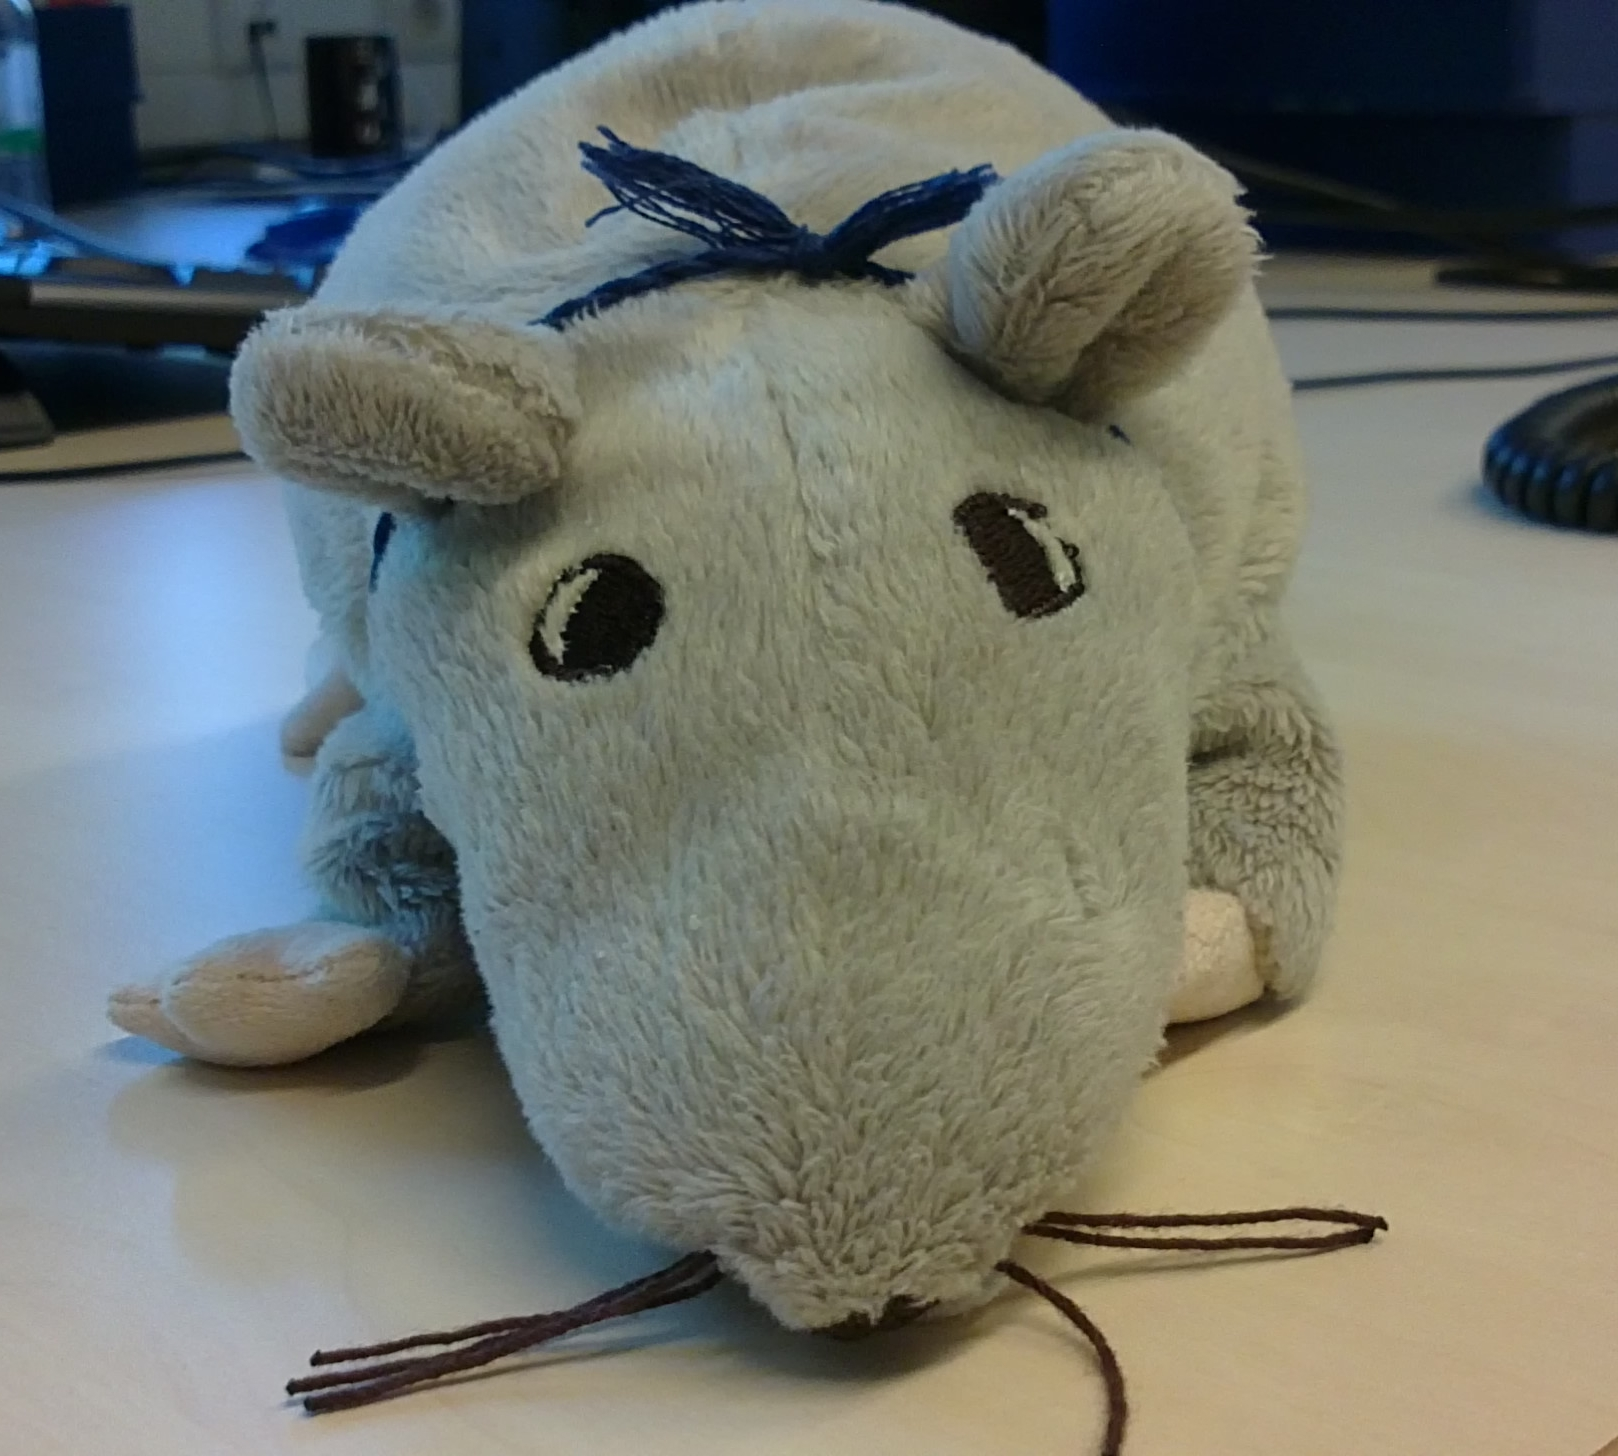
\includegraphics[width=0.8\linewidth]{pictures/ratte.jpg}
	\end{center}
	\caption{Proseminar supervisor's pet.}
	\label{fig:rat}
\end{figure}

\end{comment}